\section{The $tV$ Model}
\label{sec:tvIntro}

So called "toy models" are ubiquitous in condensed matter physics. These describe a complex system in simple terms so that attention can be given to an underlying mechanism of such system. The Ising model, in it simplest form, can describe how a system spontaneously becomes a ferromagnet by considering interactions between quantum spins and tuning an external temperature. Similarly, the Hubbard model considers the interaction strength of electrons on a lattice and a hopping rate to describe the transition between conductor and insulator. The fact that the two aforementioned examples mention phase transitions is not mere coincidence. 

Near a phase transition, evidence seems to point out to the fact that the behavior of a system is determine by a small set of parameters, a phenomenon known as universality. The size of a lattice could be one of these parameters, perhaps it could be the number of elements, or maybe even symmetry properties. Different systems having the same value for such universality parameters are said to fall under the same universality class. 

This studies that will be presented in this thesis shall be concerned with a specific model, which shall be referred to as the $tV$ model. The $tV$ model describes $N$ itinerant fermions on a 1D lattice of size $L$. These fermions can tunnel to neighboring sites and the rate at which they do so is proportional to a hopping parameter $t$. An interaction potential, $V$, between the fermions is also considered, which could be repulsive ($V > 0$) or attractive ($V < 0$). Periodic and anti-periodic boundary conditions will be assumed for the case of odd and even particles, respectively. Mathematically, this is represented by the following Hamiltonian:
%
\begin{equation}
H = -t \sum_{i} \left ( c_{i}^{\dag} c_{i+1} + c_{i+1}^{\dag} c_{i} \right )+ V \sum_{i} n_i n_{i+1}   
\label{eq:tvHamiltonian}
\end{equation}
%
where $c_{i}^{\dag}$ ($c_{i}$) creates (annihilates) a fermion on site $i$ and $n_{i}$ counts the number of fermions on site $i$. In the case that there exists a fermion on site $i$ already, then $c_{i}^{\dag} = 0$ in order to satisfy Pauli's Exclusion Principle. The interaction term can then be understood conceptually as adding to the potential energy of the system if there are multiple particles in neighboring sites. Conceptually, the first term may be more difficult to understand in its current representation, due to this operator being non-diagonal. Nevertheless, expressing it in the momentum basis, which is diagonal, will illustrate that how contributions to the kinetic energy will come from all particles with nonzero momentum (which will be all of them unless $t=0$). A detailed mapping of the kinetic energy operator from lattice site to momentum basis can be seen in Appendix \ref{appendix:kineticMapping}.

test Eq.~(\ref{eq:tvHamiltonian})

%%%%%%%%%%%%%%%%%%%
\begin{figure*}[thp]
\begin{center}
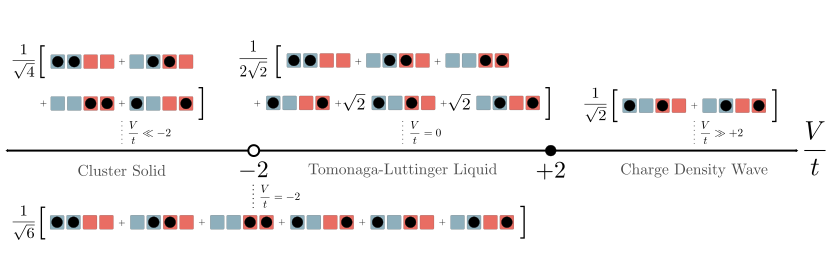
\includegraphics[width=1.0\textwidth]{phaseDiagramTV.pdf}
\end{center}
\caption{Phase diagram of the $t-V$ model accompanied by pictures of candidate ground states for $N=2$ fermions on a $L=4$ site lattice. For the purposes of measuring accessible entanglement, the lattice has been bipartitioned into spatial subregions $A$ (blue) and $B$ (red), each of size $\ell = 2$. We assume periodic boundary conditions. In the limit of strong attractive interactions where $V/t \ll -2$, the particles cluster together and there are $L$ equally probable configurations corresponding to all translations of the cluster.  At the first order phase transition where $V/t = -2$, all ${L}\choose{N}$ configurations are equally probable resulting in a flat state. In the TLL phase with $|V/t| < 2$,  particles are delocalized and we have included a characteristic state corresponding to free fermions $(V=0)$. In the limit of strong repulsive interactions where $V/t \gg 2$, fermions maximize their distance from each other resulting in a charge density wave (CDW) phase. The open and closed circles on the $V/t$ axis denote a first order and continuous phase transition, respectively.}
\label{fig:phaseDiagram}
\end{figure*}
%%%%%%%%%%%%%%%%%

Figure \ref{fig:phaseDiagram} shows the phase diagram of the $tV$ model. For $V/t \ll -2$, the fermions cluster together due to the strong attractive interaction. The state in this regime is an equal superposition of all possible such cluster configurations over all lattice sites. At $V/t = -2$, the system undergoes a second order phase transition into the Tomonaga-Luttinger Liquid (TLL) phase. Here, the state is in a superposition of all possible configurations of the fermions on the lattice. The weights for these configurations are in general different and can only be exactly known at $V/t = 0$ \cite{PhysRevLett.121.150501}. At $V/t = 2$, the system undergoes a continuous phase transition into the charged density wave (CDW) phase. At $V/t \gg 2$, the strong repulsion between particles leads to them forming an alternating pattern of particle-vacancy-particle-vacancy \dots The state in this regime becomes an equal superposition of the only two possible such configurations.

Notice that in Figure \ref{fig:phaseDiagram} the lattice sites have two different colors, blue and red. This is to illustrate that a system can be partitioned into smaller subregions. In this particular example, each partition would be of size 2 lattice sites. In fact, subdividing a system into this smaller subsystems will be necessary for the main phenomenon of interest in this thesis: quantum entanglement. The bulk of this work will consist on quantifying the amount of entanglement of a system via entropy measures. Before getting to explaining entanglement, in the next section, an overview of entropy or information measures will be given.

\section{Information measures}
\label{sec:informationMeasures}

	The probabilistic nature of quantum mechanics, provides an ideal test bed for entropy measures. In section \ref{sec:tvIntro}, it was mentioned that knowing something about $A$, will give you information about its entangled pair $B$. The amount of information gained in such measurement can be quantified by the entropy of the system. Recall that, in essence, entropy is a measure directly proportional to the disorder of a system. Thus, doing a measurement on a high entropy state, will give more information than in a highly ordered state, in which the outcome of the measurement is more like to be known a priori. For this reason, these will be referred to as information of this work for the remainder of this work.
	
	In this section, the information measure from which the ones that will be used to quantify entanglement will be introduced. Then, the actual measures of entanglement will be presented.
	
	\subsection{Shannon entropy}
	
	The Shannon or information entropy is the average amount of information gained from a a data set in which the entries occur according to some probability distribution. It is defined as:
	%
	\begin{equation}
	S = -\sum_{i} p_i \log_{b} p_i
	\label{eq:shannonEntropy}
	\end{equation}
	%
	where the sum is carried over all entries in the data set and $p_i$ is the probability of measuring entry $i$. The base $b$ can be chosen arbitrarily depending on the context. The base will be chosen as the number $e$ such that $\log_b \to \ln$ for the remainder of this work. Up next, a common day example will be presented in order to give some intuition about how information gain can be estimated with Eq.~\eqref{eq:shannonEntropy}
	
	Consider a regular coin flip. Disregarding all physical effects that can somehow bias the outcome, it is expected that either heads or tails will randomly be with equal probability $1/2$. Then, since there is no bias towards any of the two possible outcomes of the coin flip, the information gain should be at a maximum. The Shannon entropy for this case is:
	%
	\begin{align}
	S &= -\frac{1}{2} \ln{\frac{1}{2}} - \frac{1}{2} \ln{\frac{1}{2}}  \nonumber\\
	&= \ln{2}  \nonumber \\
	S &\approx 0.6931 \nonumber \dots
	\end{align}
	Now, consider a coin that has been modified in such a way that it is more likely to get one outcome than the other. For the sake of this example, let's say that heads shall occur with probability $2/3$, while tails with $1/3$. Then, since it is two times more likely that heads will occur instead of tails, more certainty about the outcome is known beforehand and thus the information gained decreases. Shannon entropy gives:
	%
	\begin{align}
	S &= -\frac{2}{3} \ln{\frac{2}{3}} - \frac{1}{3} \ln{\frac{1}{3}} \nonumber \\
	S &\approx 0.6365 \dots \nonumber
	\end{align}
	%
	Finally, an extreme case would be a coin that was incorrectly manufactured and has heads on two sides. Opposite to a regular coin, in which maximum information is gained because both heads and tails have the same probability, the probability for heads to land in this case is 1, while 0 for tails. Since the result is already known before the coin flip, the information gain after the coin flip is none. Shannon entropy gives:
	%
	\begin{align}
	S &= -1\ln{1} = 0 \nonumber
	\end{align}
	%	

	Now that some intuitive examples were discussed, the quantum information theory counterpart of Shannon's entropy will be presented.
	
	\subsection{von Neumann entropy}
	
	In quantum statistical mechanics, the probabilities of measuring a state are encoded within its density matrix. The density matrix is defined as:
	%
	\begin{align}
	\label{eq:densityMatrix}
	\rho = \vert \Psi \rangle \langle \Psi \vert
	\end{align}
	%
	In quantum information theory, Shannon entropy maps to the von Neumann entropy:
	%
	\begin{equation}
	S = -\Tr\rho_{A} \ln{\rho_A}
	\label{eq:vonNeumannEntropy}
	\end{equation}
	%
	where $\rho_A$ is the reduced density matrix of subsystem $A$. The reduced density matrix of $A$ is obtained by tracing out the degrees of freedom of $B$:
	%
	\begin{equation}
	\rho_{A} = \Tr_B \rho = \sum_b \langle \psi_b \vert \Psi \vert \psi_b \rangle
	\label{eq:partialTrace}
	\end{equation}
	%
	where the sum is carried over all possible states in which subsystem $B$ can be in.
	
	\subsection{R\'enyi entropy}

	
\section{Quantum entanglement}
\label{sec:quantumEntanglement}

	A quantum many body system is entangled if its constituents present correlations that cannot be classically described. In other words, assuming subsystems $A$ and $B$ are entangled with one another, knowing something about $A$ automatically gives you some knowledge of $B$. These subsystems can represent subsets of particles, spatial subregions, or just some quantum mode in general, such as momentum. An overview of each of these type of partitions will now be given.

	\subsection{Particle entanglement}
	
	The particles of a quantum many body system can be given labels, such that subsets of particles in the system that share a common label can be considered as a subsystem. Then, the particle partitioned entanglement can be quantified. 
	
	Mathematically,  if a system is entangled or not can be determined by rewriting the state of the system in terms of the states of each subsystem $A$ and $B$. If the overall state cannot be factored into tensor products of the states of $A$ and $B$, then the system is entangled. The condition for entanglement of $A$ and $B$ is then:
	
	\begin{equation}
	\vert\Psi\rangle \neq \vert\Psi_{A}\rangle \otimes \vert\Psi_{B}\rangle
	\label{eq:entanglementCondition}
	\end{equation}
	
	$\vert\Psi_{A}\rangle$ and $\vert\Psi_{B}\rangle$ represent the states of subsystems $A$ and $B$, respectively. Formally, the state $\vert\Psi_{A}\rangle$ is a vector space that exists in Hilbert Space $A$, and likewise for $B$, such that the full Hilbert Space of the system is a tensor product of the subspaces: $\mathcal{H} = A \otimes B$.
	
	Due to the indistinguishability of particles, the $n$-body reduced of the ........
	
	\begin{equation}
	\rho_{n} = \int dx_n \dots \int dx_1 \langle x_1 \dots x_n \vert\Psi\rangle \langle\Psi\vert x_1 \dots x_N \rangle
	\label{eq:nBodyDensityMatrix}
	\end{equation}
	
	
 	
	\subsection{Spatial and mode entanglement}
	
	\subsection{Accessible Entanglement}



	

	
